\section{Nonlinear Analysis}
In this section the nonlinear nature of the system is studied.\fxnote{name the tools used in the section}

It is possible to map trajectories in the ($\theta$, $\dot{\theta}$)-plane assuming no applied force. To construct the phase portrait the dynamic equations, \autoref{eq:dynamicEquation1} and \autoref{eq:dynamicEquation1}, are combined. First $\ddot{x}$ is isolated in \autoref{eq:dynamicEquation2},
%
\begin{flalign}
  \ddot{x} &= - \frac{m l \cos \theta \ddot{\theta}}{M + m}  + \frac{m l \sin \theta \dot{\theta}^2}{M + m} + \frac{f}{M + m}   \ \ \ . & %\unit{N \cdot m}
  \label{eq:dynamicEquationX}
\end{flalign}

This expression for $\ddot{x}$ is then substituted in \autoref{eq:dynamicEquation1} to obtain the dynamics in therms of the angle and its derivatives.
%
\begin{flalign}
  m l \cos \theta
  \left(
    - \frac{m l \cos \theta \ddot{\theta}}{M + m}  + \frac{m l \sin \theta \dot{\theta}^2}{M + m} + \frac{f}{M + m}
  \right)
  + m l^2 \ddot{\theta} - m l g \sin \theta &=  0   \ \ \ . & %\unit{N \cdot m}
  \label{eq:dynamicEquationSubsX}
\end{flalign}

Rearranging yields,
%
\begin{flalign}
  \left( m l^2 - \frac{m^2 l^2}{M + m} \cos ^2 \theta \right) \ddot{\theta}
  + \left( \frac{m^2 l^2}{M + m} \sin \theta \cos \theta \right) \dot{\theta}^2
  + f \frac{m l}{M + m} \cos \theta - m g l \sin \theta &=  0   \ \ \ , & %\unit{N \cdot m}
  \label{eq:alphaBetaGamma}
\end{flalign}
%
which is the reduced system on the general form,
%
\begin{flalign}
  \alpha (\theta) \ddot{\theta} + \beta (\theta) \dot{\theta}^2 + \gamma (\theta) &=  0   \ \ \ , & %\unit{N \cdot m}
  \label{eq:alphaBetaGammaGeneral}
\end{flalign}
%
where, $\alpha (\theta)$, $\beta (\theta)$ and $\gamma (\theta)$ are the scalar functions of $\theta$ from \autoref{eq:alphaBetaGamma}.

Finally the reduced system on state space form, where $x_1 = \theta$ and $x_2 = \dot{\theta}$,
%
\begin{flalign}
  \dot{x_1}  &=  x_2  \nonumber \\
  \dot{x_2}  &=  -\frac{\beta (x_1)}{\alpha (x_1)} x_2^2 -\frac{\gamma (x_1)}{\alpha (x_1)}   \ \ \ . & %\unit{N \cdot m}
  \label{eq:stateSpaceThetaDynamics}
\end{flalign}

In \autoref{fig:phasePortrait} the phase portrait is generated using pplane8.\fxnote{remove pplane8, redo plots}

\begin{figure}[H]
  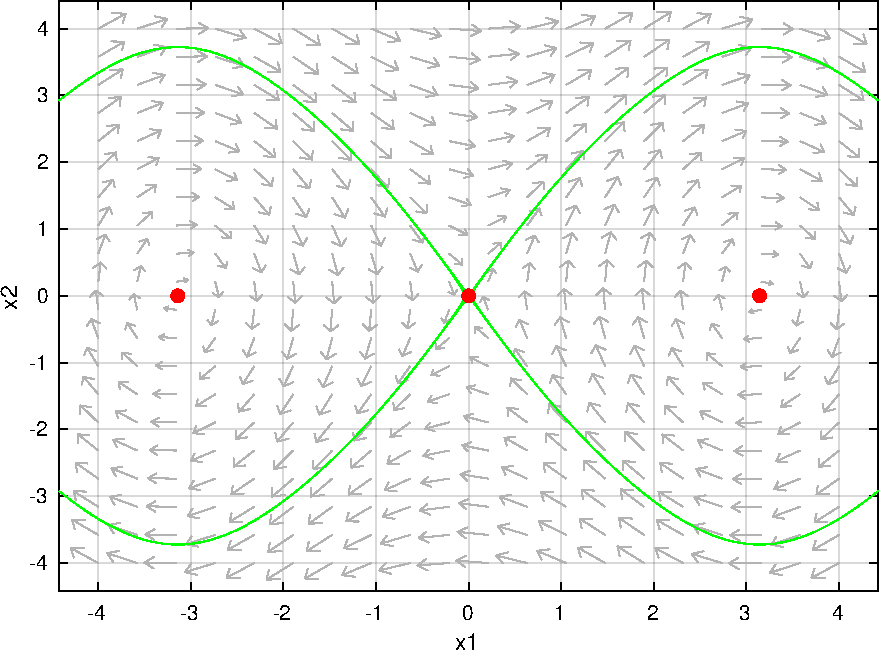
\includegraphics[width=.8\textwidth]{figures/systemPhasePortrait}
  \caption{Phase portrait of the $\theta$-dynamics, where $x_1 = \theta$ and $x_2 = \dot{\theta}$. The equilibrium points are shown in red and the unstable orbits at the saddle point are indicated in green.}
  \label{fig:phasePortrait}
\end{figure}

As there is no friction in the system the pendulum will maintain one particular orbit around one of the center equilibrium points so long as the initial value is within the confines of the unstable orbit at the saddle point. This means that the pendulum will oscillate without loss of amplitude if the initial angular velocity, $\dot{\theta}$, is zero or at least places the starting point within the saddle.\\
If on the other hand the initial value of $\dot{\theta}$ is positive and $\theta$ is zero (upright position), then the pendulum will do full rotations around the cart, thus continuously increasing the angle.

If a force is imposed on the system it can change the phase portrait, allowing for other possible trajectories. This is further investigated in the following chapter.
